% 原书PDF第83页4.5.3起至第88页4.6前，包含表4.13和表后3行。
\subsection{线性调控网络}
第4.5.2节研究了低秩表示诱导的因果网络，可用于评估通路或基因集合之间的调控关系。下一步是估计一条或多条通路内部基因的调控网络。若将 RNA-seq 表达数据视为函数曲线，则以曲线为节点的因果网络估计将在第5章讨论，因为 RNA-seq 与甲基化数据均可视为函数曲线。第5章将发展函数值性状的因果推断统计方法，并应用于 RNA-seq 与甲基化因果网络。

若基因表达由微阵列测量，或用汇总统计量表示 RNA-seq 表达，则可用第2.4节介绍的统计方法估计因果网络。相应算法能够构建包含数百个基因的调控网络，再将这些估计的子网络整合为全基因组调控网络。

\subsection{非线性调控网络}
第2.5.1节发展了用于双变量因果发现的函数模型，以及用于因果网络发现的非线性结构方程，两者均可估计非线性调控网络。与相关分析通过相关系数评估一对基因的共表达类似，可以用双变量因果发现的函数模型研究两个基因的因果关系，发现因果结构。通过评估成对的因果效应关系，可以构建因果网络。

\begin{bookexample}{4.9}
为评价性能，下面用例4.9说明如何以加性噪声模型检验一对变量的因果关系。先考虑噪声服从正态分布的非线性函数加性噪声模型，用二维模型模拟数据（Nowzohour and Bühlmann 2016）：
\[
\begin{aligned}
X&=\varepsilon_1,\\
Y&=X+b\log(X)+\varepsilon_2,
\end{aligned}
\]
其中参数 $b\in[-1,1]$ 控制模型的线性程度，噪声 $\varepsilon_1,\varepsilon_2$ 服从正态分布 $\varepsilon_k\sim N(0,100)$。两个变量之间三种可能的因果关系，生成下列模型（Nowzohour and Bühlmann 2016）。

\noindent 模型1：$X$ 导致 $Y$。
\[
X=\varepsilon_1,\qquad Y=f(x)+\varepsilon_2.
\]
\noindent 模型2：$Y$ 导致 $X$。
\[
X=g(Y)+\varepsilon_1,\qquad Y=\varepsilon_2.
\]
\noindent 模型3：$X$ 与 $Y$ 独立。
\[
X=\varepsilon_1,\qquad Y=\varepsilon_2.
\]
用第2.5.1.1节的加性噪声模型，在三个模型中选择一个，并用 B 样条拟合函数模型。图4.23给出了正态误差下的误判率。$b=0$ 时模型为线性，误判率接近0.5，相当于随机猜测。当 $b$ 偏离零时，模型变为非线性，误判率接近零，表明非线性模型下有较高概率作出正确因果推断。

再考察误差非正态的线性模型，按下式模拟：
\[
X=\varepsilon_1,\qquad Y=X+\varepsilon_2.
\]
噪声服从
\[
\varepsilon_k=\operatorname{sgn}(v_k)|v_k|^q,\qquad v_k\sim N(0,25),
\]
其中 $q\in[0.5,2]$ 控制高斯性（Nowzohour and Bühlmann 2016）。再次用 B 样条拟合非线性函数，以加性噪声模型评估因果性。误判率见图4.24。当模型线性且误差正态（$q=1$）时，错误因果推断的概率很高；即使模型线性，只要误差非正态（$q$ 偏离1），仍有较高概率作出正确推断。
\end{bookexample}
\begin{figure}[htbp]
\centering
\begin{tikzpicture}[x=1cm,y=1cm]
\node[anchor=south west,inner sep=0] at (0,0) {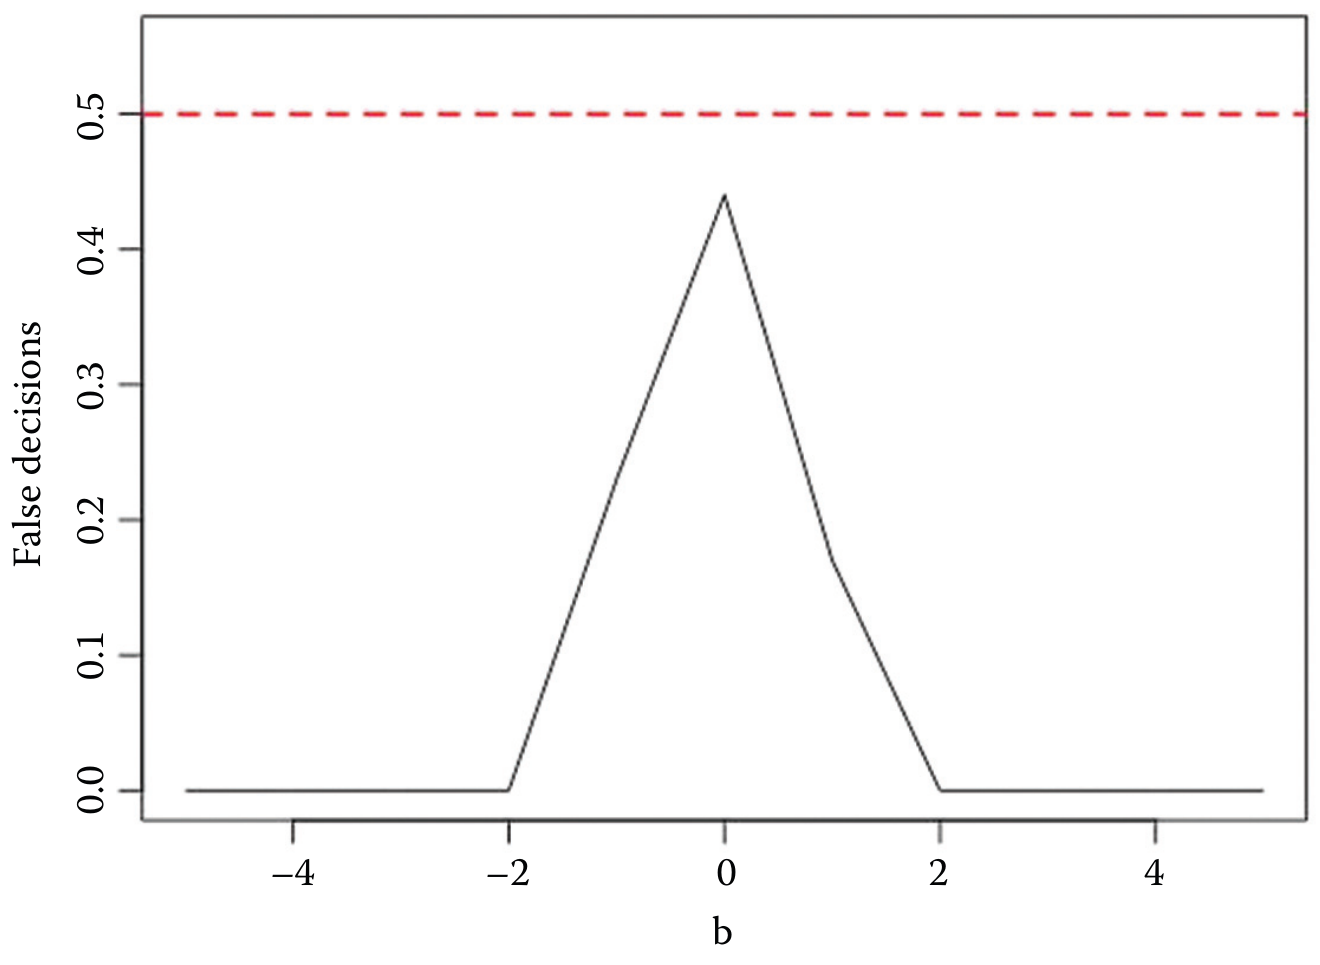
\includegraphics[width=11.5cm]{figures/ch04a_fig23_data.png}};
\fill[white] (0.0585,3.4352) rectangle (0.4569,5.6369);
\node[inner sep=0pt,fill=white,rotate=90,font=\fontsize{8}{8}\selectfont] at (0.2577,4.5360) {误判率};
\end{tikzpicture}
\origfig{23}{假定非线性模型及正态误差分布时，双变量因果发现的误判率。}
\label{fig:ch04a-23}
\end{figure}

\begin{figure}[htbp]
\centering
\begin{tikzpicture}[x=1cm,y=1cm]
\node[anchor=south west,inner sep=0] at (0,0) {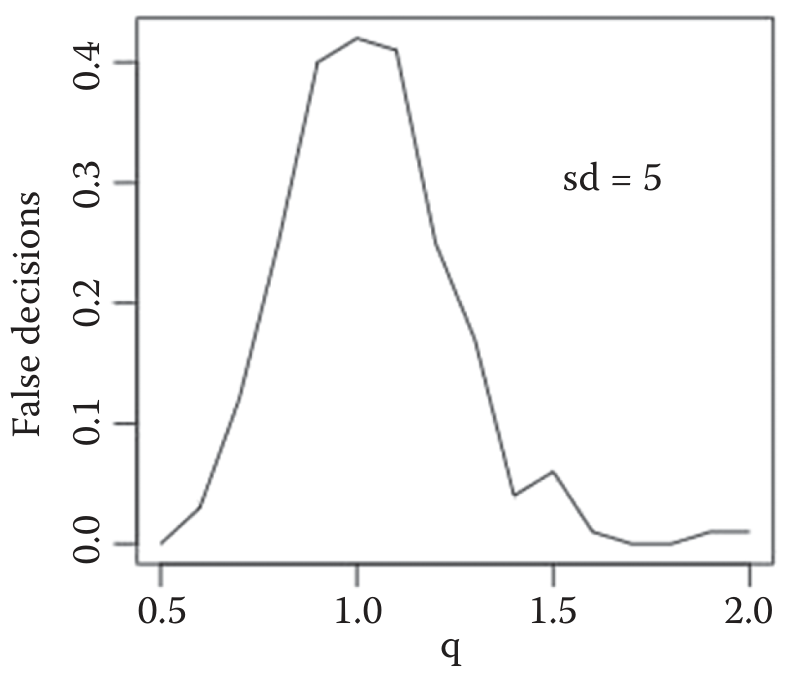
\includegraphics[width=9.5cm]{figures/ch04a_fig24_data.png}};
\fill[white] (0.0824,2.9062) rectangle (0.6164,5.9451);
\node[inner sep=0pt,fill=white,rotate=90,font=\fontsize{8}{8}\selectfont] at (0.3494,4.4257) {误判率};
\fill[white] (6.7848,5.7832) rectangle (8.0425,6.3172);
\node[inner sep=0pt,fill=white,rotate=0,font=\fontsize{8}{8}\selectfont] at (7.4137,6.0502) {标准差=5};
\end{tikzpicture}
\origfig{24}{假定线性模型及非正态误差分布时，双变量因果发现的误判率。}
\label{fig:ch04a-24}
\end{figure}


\begin{bookexample}{4.10}
为说明基因调控网络估计的应用，将非线性加性噪声模型与用于共表达网络构建的 glasso，应用于447个组织样本、79个基因的 Wnt 信号通路 RNA-seq 数据。双变量因果发现的函数模型估计出49个方向，见图4.25。蓝色表示与 KEGG 通路数据库中方向相同的共同边；绿色表示估计路径与 KEGG 中有直接效应的路径相同；红色表示与有间接效应的路径相同；棕色表示 KEGG 中的结合／关联；灰色表示 KEGG 中不存在该估计方向；深红色表示估计边在 KEGG 中具有相反方向。函数模型、glasso 与随机网络的检出功效见表4.13。结果表明，用于基因调控网络估计的非线性函数模型，比 glasso 更为精确。
\end{bookexample}
\begin{figure}[p]
\centering
\fbox{\begin{minipage}{.92\linewidth}\small
前129个方向全部从 Wnt3A 与 Dkk4 出发。下图展示前50个方向，以及从 Wnt5 和 Wnt11 出发或指向它们的其他显著方向。
\end{minipage}}
\par\medskip
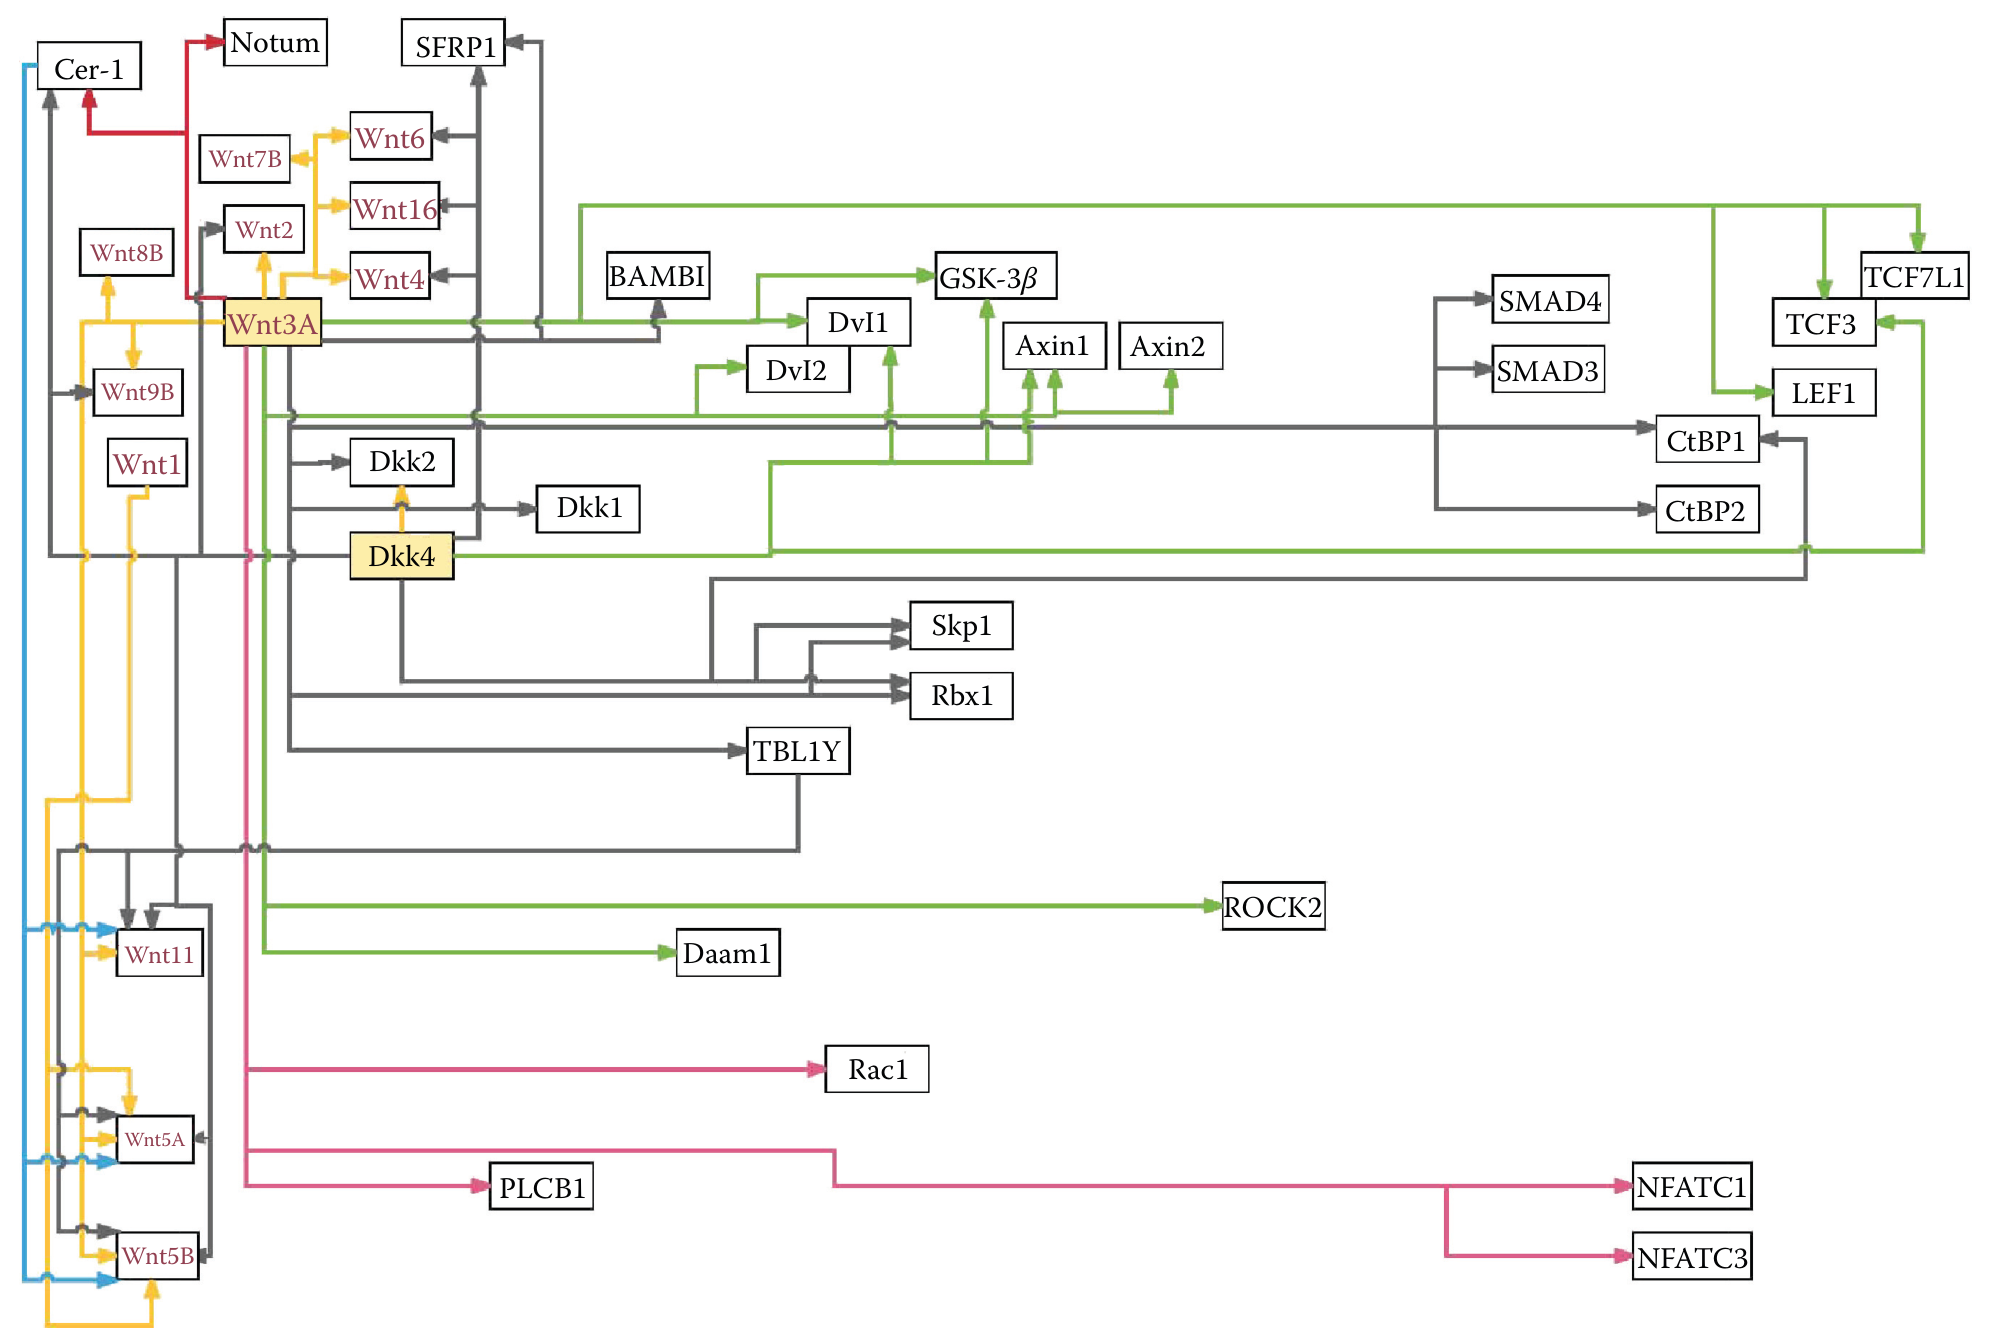
\includegraphics[width=13.8cm]{figures/ch04a_fig25_data.png}
\par\smallskip
\begin{tikzpicture}[x=1cm,y=1cm,font=\footnotesize]
\fill[fill={rgb,255:red,201;green,48;blue,72}] (0,2.10) rectangle (.65,2.32);
\node[anchor=west,inner sep=0] at (.85,2.21) {KEGG 中存在相反方向};
\fill[fill={rgb,255:red,144;green,144;blue,143}] (0,1.68) rectangle (.65,1.90);
\node[anchor=west,inner sep=0] at (.85,1.79) {KEGG 通路中未显示关联};
\fill[fill={rgb,255:red,255;green,198;blue,75}] (0,1.26) rectangle (.65,1.48);
\node[anchor=west,inner sep=0] at (.85,1.37) {存在关联，可据此建立潜在方向};
\fill[fill={rgb,255:red,233;green,88;blue,133}] (0,0.84) rectangle (.65,1.06);
\node[anchor=west,inner sep=0] at (.85,0.95) {KEGG 虚线通路中至少存在一个方向};
\fill[fill={rgb,255:red,119;green,188;blue,67}] (0,0.42) rectangle (.65,0.64);
\node[anchor=west,inner sep=0] at (.85,0.53) {KEGG 实线通路中至少存在一个方向};
\fill[fill={rgb,255:red,89;green,193;blue,224}] (0,0.00) rectangle (.65,0.22);
\node[anchor=west,inner sep=0] at (.85,0.11) {KEGG 中存在直接方向};
\end{tikzpicture}
\origfig{25}{推断得到的 Wnt 信号通路调控网络。}
\label{fig:ch04a-25}
\end{figure}

\begin{table}[htbp]
\centering
\origtable{13}{非线性因果推断的检出功效}
\begin{tabular}{lcc}
\toprule
&\multicolumn{2}{c}{检出功效}\\
\cmidrule(lr){2-3}
方法&有向路径&不考虑方向的路径\\
\midrule
函数模型&38\%&46\%\\
Glasso&X&24\%\\
随机网络&X&32\%\\
\bottomrule
\end{tabular}
\end{table}

\FloatBarrier
